\cotefile{157-2}
\scanpage{99}
\mspage{43}
% archive sheet number: 98
les inclusions

\[
 X_s\longrightarrow {}_{s\backslash}X_{\deleted{\unsure{/s|s}}},\quad X_s\longrightarrow X_{/s}\quad\deleted{\unsure{{}_{s\backslash}X_s}}
\]

et de $=$ pour $Y$, sont des $W_{\infty}$-équiv. donc des $W$-équiv.
% slanted
\margin{comparer déf.~3 p.~117 \unsure{du|de} (I)}
(Il suffirait $=$ que $X,Y$ soient des $W$-fibrations \deleted{\unsure{faibles}} sur $S$*, i.e. \deleted{par déf.} que les foncteurs précédents soient des $W$-équivalences, et que \deleted{ils soient des \unsure{équiv.}} \inserted{la $=$ condition soit satisfaite} après tt chgt. de base sur $S$), l'argument \unsure{dans le cas} lisse resp. propre montre déjà que

\diagram{\begin{tikzcd}[ampersand replacement=\&,column sep=small,row sep=small]
 c \& b\arrow[l,Rightarrow]\arrow[r,Leftrightarrow]\arrow[d,Rightarrow] \& c'\\
 \& a \&
\end{tikzcd}}

% slanted
\margin{valable en supposant seulement $X,Y$ des $W$-\unsure{fibrissimes|fibrissures}.}

, et que la $W$-équivalence par fibres \deleted{implique} (ou la $W$-\deleted{\unsure{équiv.}} locale sur $S$, resp. bilocale sur $(\,)$) implique déjà la $W$-équivalence \uline{universelle} sur $S$.

La question $a)\Rightarrow b)$ est par contre \unsure{nettement|nullement} plus délicate, et on a vu que ce n'est \deleted{pas} nullement le cas pour tout \unsure{localisateur|localiseur} fondamental -- sans doute pas pour celui associé au dérivateur $\mathrm{Der}(\mathbb Z\text{-}\unsure{\mathrm{Mod}|\mathrm{Modules}})$, en tous cas pas à celui associé à $\mathrm{Der}(k\text{-}\mathrm{Mod})$, quand $2$ est inv. dans $k$. (Il suffirait $=$ \deleted{\unsure{que un}} que $\exists n\in\mathbb N,\ n\geq 2$, tel que $n$ inv. dans $k$ -- le contrexemple typique est

\diagram{\begin{tikzcd}[ampersand replacement=\&,row sep=tiny,column sep=small]
 S^1\arrow[r,"n"]\arrow[d,equal] \& S^1\arrow[d,equal]\\
 X \& Y=S
\end{tikzcd}}

, le rev. étale d'ordre $n$ d'un cercle. \inserted{L'implication $a\Rightarrow b$} \deleted{\unsure{C'}}est \inserted{donc} une condition très forte sur $W$, je vais la noter $\mathrm L\,5$ (l'ancienne L5 \unsure{``$3^{\mathrm e}$''}, cf page 2, \deleted{\unsure{que}} ne \unsure{méritant|méritait} pas de survivre, car c'est \unsure{une} côte mal taillée)

% slanted
\margin{Dans \uline{XII} (p.~12) on voit que si $W$ satisfait à L1, \inserted{L3 quater}, L4 bis (cf. p.~\unsure{suivante}), L5, alors \unsure{vraiment} $\boxed{W=W_{\infty}}$ ! Donc c'est vraiment en \unsure{supprimant|supposant} \unsure{l'hyp.} \unsure{L5} qu'on \unsure{s'aventure} \unsure{hors} du train-train}

\uline{L 5} Soit

\diagram{\begin{tikzcd}[ampersand replacement=\&,column sep=small,row sep=tiny]
 X\arrow[rr,"f"]\arrow[dr] \& \&Y\arrow[dl]\\
 \&S\&
\end{tikzcd}}

dans $\mathrm{Cat}$, avec $X,Y$ des \unsure{Hot}-fibrés sur $S$. Si $f$ est une \deleted{\unsure{Hot}} $W$-équiv. \inserted{(``grossière'' p.r. à $S$)} alors c'est une $W$-équivalence par fibres.

On a vu qu'à un $\varepsilon$ près (\unsure{``lemme''} p.~23), L5 est une conséquence de

\uline{L 6} \deleted{\unsure{le foncteur}} Soit $f:X\longrightarrow Y$ une $W$-équivalence, $Y'\longrightarrow Y$ \deleted{une} \inserted{morphisme parfait, (\unsure{c.à.d.} lisse et propre)} \deleted{\unsure{Hot-fibration}}, alors $f':X'=X\times_Y Y'\longrightarrow Y'$ est une $W$-équiv.

\scanpage{100}
\mspage{\deleted{\unsure{43}}44}
% archive sheet number: 99
Notons la variante bien naturelle

\uline{L 6} \uline{bis} : Comme L6, \deleted{\unsure{avec}} mais en supposant seulement $Y'\mathbin{\unsure{-|\to}}Y$ une $\mathrm{Hot}$-fibration.

Il y a des chances que \inserted{pratiquement,} quand L6 (ou seulement L5) est vérifié, L6 bis l'est aussi.

On va introduire un axiome

\uline{L 7} a) \unsure{Soient|Soit} $(f_i:X_i\mathbin{\unsure{-|\to}}Y_i)_{i\in I}$ une famille de flèches de $\mathrm{Cat}$, soit $f:\coprod X_i\longrightarrow\coprod Y_i$ la flèche \deleted{\illegible{1}} corr. sur les catégories sommes. Pour que $f\in W$, \deleted{\unsure{on}} il f. et s que $f_i\in W$ pour tt $i\in I$.

b) Soit $f:X\longrightarrow Y$ dans $W$. Si $Y$ est $0$-connexe, $X$ aussi.

Cet axiome équivaut à la conjonction de \unsure{L o)|L a)} ($f\in W\Longrightarrow\pi_0(f)$ bijectif) et de la validité du ``lemme'' page 23, que je \unsure{remets|recopie|récris} ici pour mémoire :

\uline{Lemme} L'axiome L7 précédent sur le localiseur fondamental $W$ équivaut : la \deleted{conjonction des} \inserted{conditions suivantes :} $f:X\longrightarrow Y$ \deleted{conditions suivantes} est dans $W$ ssi $\pi_0(f)$ est bijectif, et \deleted{\unsure{a')|ii)}} $f$ induit des $W$-équivalences $f_i:X_i\mathbin{\unsure{-|\to}}Y_i$ sur les composantes connexes.

Il me faut revenir encore sur le 1) de la proposition, il n'est pas vrai que \deleted{se réduise à} \inserted{``c'est''} la condition L4 \deleted{sur} $W$ (que j'admettais, ai-je dit), c'est L4 dans le cas particulier où $Y=S$. Réflexion faite, je la vois comme une variante renforcée de L4, qui ne semble pas \unsure{devoir} découler de L4 ; \deleted{\unsure{Soit quoi} C'est une variante affaiblie de \unsure{l'én.}}

\uline{L 4 bis} Soit $f$ :

\diagram{\begin{tikzcd}[ampersand replacement=\&,column sep=small,row sep=tiny]
 X\arrow[rr]\arrow[dr] \& \& Y\arrow[dl]\\
 \& S\&
\end{tikzcd}}

, \deleted{\unsure{suppos}} dans $\mathrm{Cat}$, supposons que \deleted{\unsure{soit}} $f$ soit une $W$-équiv. \uline{loc. sur} $S$ (i.e. $f_{/s}:X_{/s}\mathbin{\unsure{-|\to}}Y_{/s}$ \unsure{une} $W$-équiv. $\forall s\in S$), alors $f$ est une $W$-équivalence.

% slanted
\margin{équivaut à l'axiome dual, \deleted{\unsure{en prenant}} \unsure{au|ou} \unsure{(cf.)} \deleted{\unsure{lieu de}} \unsure{que} \deleted{\unsure{cela signifie que les foncteurs|en prenant les catégories opposées}}}

\scanpage{101}
\mspage{45}
% archive sheet number: 100
\unsure{Pour|Par} la suite, \unsure{par} un ``localiseur fondamental'', nous entendrons un ens.

\[
 W\subset\mathrm{Fl}\,\mathrm{Cat}
\]

satisfaisant \inserted{(tout au moins)} les axiomes

\[
 \mathrm L1,\ \mathrm L3\ \text{quater},\ \mathrm L4\ \text{bis},\ \mathrm L7
\]

i.e. \deleted{\unsure{satisferaient les}}

\noindent\begin{minipage}{.035\linewidth}
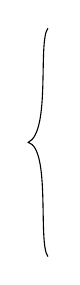
\begin{tikzpicture}
\draw (0.25,1.45) .. controls (0.12,1.28) and (.29,.14) .. (0,0) .. controls (.29,-.08) and (.12,-1.28) .. (.25,-1.45);
\end{tikzpicture}
\end{minipage}\begin{minipage}{.93\linewidth}
a) \uline{Saturation} de $W$ (cond. a) b) c) p.~1)

b) $W_\infty\subset W[\subset W_0]$\inserted{cf d)}

c) Si $f:X\longrightarrow Y$ sur $S$ est loc. sur $S$ une $W$-équiv., alors $f\in W$ \inserted{(L4 bis)}

d) Pour que $f:X\longrightarrow Y$ soit dans $W$, il f. et s. que $\pi_0(f)$ soit bijectif, et que les $f_i:X_i\longrightarrow Y_i$ induits sur les compos. conn. soient dans $W$.
\end{minipage}

% slanted
\margin{Je ne suis plus sûr s'il est vraiment utile d'imposer $W_\infty\subset W$. \deleted{\illegible{1}} Prendre au \deleted{lieu de} ça l'axiome de l'objet final, \unsure{soit b')|L iv bis b')}. Si on veut a) b') c) + L5, alors on aura $W\subset\unsure{W_\infty}$.}

% slanted
\margin{\uline{NB} a) b) c) + L5 implique $W=W_\infty$, cf annotation page 43.}

\deleted{Par contre, les \unsure{axi}} Ces axiomes sont vérifiés par tous les $W$ que je connais, et qu'on aurait envie de regarder comme localiseurs. Par contre, L5, L6, L6 bis (p.~43,44) sont des axiomes de nature beaucoup plus spéciale, j'ai envie de dire qu'ils distinguent les localiseurs de nature proprement ``\uline{homotopique}'' de ceux qui sont de nature ``\uline{homologique}'' (ou ``cohomologique''). Il faudrait que je m'assure qu'ils sont satisfaits pour les $W_i$ ($i$-équiv. d'homotopie).

% slanted
\margin{C'est \uline{faux}, cf annotation ci-dessus}

Le fait que L4 bis \inserted{i.e c) ci-dessus} implique l'axiome dual résulte du fait \deleted{que si $f:X\longrightarrow Y$, $f\in W$} que L4 bis implique ceci

\uline{Proposition 2} Soit $f:X\longrightarrow Y$ dans $\mathrm{Cat}$, alors $f\in W$ ssi $f^o:X^o\mathbin{\unsure{-|\to}}Y^o$ est dans $W$.

Se voit par l'argument de I, page 75 Corr.~2) -- n'utilise que L4, pas $=$ L1, L3.

\scanpage{102}
\mspage{46}
% archive sheet number: 101
Je vais essayer de résumer ce que je crois avoir compris :

1) La $W$-équivalence ``par fibres'' n'a d'intérêt \deleted{\unsure{que dans les}} (pour construire des cat. localisées) que dans le cas où on sait qu'elle implique déjà, soit la $W$-équiv. locale, soit la $W$-équivalence colocale. (soit $=$ la $W$-équiv. universelle) sur $S$, donc quand on suppose $X,Y$ pour le moins \inserted{tous deux} soit $W$-lisses, soit $W$-propres, soit $W$-fibrés sur $S$.

2) On pourrait appeler la $W$-équivalence locale sur $S$ la ``$W$-\uline{équivalence fine à gauche}'' \inserted{sur $S$}, et la $W$-équivalence colocale sur $S$ la ``\uline{$W$-équivalence fine à \deleted{\unsure{gauche|dr}}droite}'' sur $S$. Elles coïncident dans $\underline{\mathrm{Fibhot}}\,S$, a fortiori dans $\underline{\mathrm{Parf}}\,S$ \deleted{\unsure{et dans les}} et dans les quatre catégories (cf diagramme p.~8)

% slanted
\margin{On pourrait les appeler les six catégories \uline{internes} du diagramme.}

$\underline{\mathrm{Fib}}_0\,S$, $\underline{\mathrm{Fibsc}}_0\,S$, $\underline{\mathrm{Cofib}}_0\,S$, $\underline{\mathrm{Cofibsc}}_0\,S$. Par contre, elles ne coïncident pas sur les catégories \uline{bordantes} du diagramme, notamment sur $\underline{\mathrm{Liss}}\,S$, $\underline{\mathrm{Prop}}\,S$, $\underline{\mathrm{Fib}}\,S$, $\underline{\mathrm{Cofib}}\,S$, $\underline{\mathrm{Fibsc}}\,S$, $\underline{\mathrm{Cofibsc}}\,S$. À cet égard, c'est la \inserted{$W$-}\uline{équivalence fine} \uuline{droite} \inserted{(en \unsure{termes|terme} des $ {}_{s\backslash}X$)} qui est intéressante sur le côté (hélas) gauche du diagramme, i.e. pour $\underline{\mathrm{Liss}}\,S$, $\underline{\mathrm{Fib}}\,S$, $\underline{\mathrm{Fibsc}}\,S$, alors que c'est la $W$-\uline{équivalence fine} \uuline{gauche} (en \unsure{termes|terme} de $X_{/s}$) qui est pertinente du côté droit, pour $\underline{\mathrm{Prop}}\,S$, $\underline{\mathrm{Cofib}}\,S$, $\underline{\mathrm{Cofibsc}}\,S$. On n'aura jamais à \deleted{\unsure{s}} regarder simultanément les deux équivalences fines sur la \deleted{\unsure{ma}} même catégorie du diagramme, à la seule exception de $\mathrm{Cat}_{/S}$ tout entier,

\scanpage{103}
\mspage{47}
% archive sheet number: 102
3) La $W$-équivalence grossière, elle, est ``bonne partout'' -- mais ça dépend pour qui. Pour les \inserted{\deleted{\unsure{tr}} 6} catégories qui sont \deleted{soit à l'intérieur, soit} au dessus de $\underline{\mathrm{Fibhot}}\,S$, i.e.

\[
 \underline{\mathrm{Fibhot}}\,S,\ \underline{\mathrm{Parf}}\,S,\ \underline{\mathrm{Fib}}_0\,S,\ \underline{\mathrm{Fibsc}}_0\,S,\ \underline{\mathrm{Cofib}}_0\,S,\ \underline{\mathrm{Cofibsc}}_0\,S,
\]

elle coïncide avec toutes les autres équivalences \unsure{$\in$|$\varepsilon$} (moyennant l'axiome L5), pour les trois catégories bordantes supérieures gauches

\[
 \underline{\mathrm{Liss}}\,S,\ \underline{\mathrm{Fib}}\,S,\ \underline{\mathrm{Fibsc}}\,S
\]

du diagramme, elle coïncide avec la $W$-équiv. fine droite, et dualement sur

\[
 \underline{\mathrm{Prop}\,S},\ \underline{\mathrm{Cofib}\,S},\ \underline{\mathrm{Cofibsc}}\,S
\]

elle coïncide \deleted{\unsure{avec}} avec la $W$-équivalence fine gauche. Quant à $\mathrm{Cat}_{/S}$ tout entier, c'est la seule des \deleted{quatorze notions} \inserted{catégories du} \deleted{de $W$-équivalence qui y donne une localisé \unsure{distincte}.} diagramme où il y ait \uline{trois} notions intéressantes différentes de $W$-équivalence\unsure{s}, à savoir : la grossière, et les deux fines (à gauche, à droite). Sur les autres \inserted{six} catégories bordantes du diagramme, il y en \deleted{\unsure{a}} en principe deux : la grossière, et une spécifiée des deux fines (défendu de regarder l'autre -- à ses risques et périls \ldots) : la droite du côté gauche, la gauche du côté droit. (NB Je devrais refaire le diagramme, décidément, en mettant les fibrations à droite, ou à gauche.) Quant aux \inserted{six} catégories internes \deleted{\unsure{au}} diagramme, dans \unsure{icelles|elles} il n'y a plus qu'une seule notion de $W$-équivalence (puisque sur elles les quatre notions coïncident).

\scanpage{104}
\mspage{\deleted{\unsure{48}}49} (\uline{NB} il n'y a pas de page 48)
% archive sheet number: 103

Je résume maintenant ce que je crois avoir compris sur les catégories localisées correspondantes. Il y en a, à équivalence près, \uline{trois} différentes seulement en tout et pour tout, quand on prend les localiseurs ``admis'' dans les catégories, comme je viens de le dire (c'était ça en somme l'intérêt objectif des prescriptions !) : \deleted{\unsure{Précision} $\mathrm{Cat}_{/S}$} \unsure{Précisons mieux|Précision première} \deleted{\unsure{donc}}

1$^\circ$) La $W$-\uline{équivalence} \uline{grossière} donne ``la même'' catégorie localisée pour les 13 catégories du diagramme, i.e. toutes les flèches de transition du diagramme induisent des équivalences pour cette $W$-équivalence \uline{grossière}. Le localisé \deleted{\unsure{correspondant}} sera noté $\boxed{\mathrm{HOT}^{\mathrm{lc}}_W(S)}$, où l'exposant lc signifie : ($W$-types d'homotopie relatifs sur $S$) ``\uline{localement constants}''.

(Il me reste quand même un petit doute pour $\underline{\mathrm{Fibsc}}\,S$ et $\underline{\mathrm{Cofibsc}}\,S$*, si l'équivalence grossière y est bel et bien \unsure{raisonnable|vraisemblable}. On verra en faisant la démonstration.)

% slanted
\margin{Ce \unsure{doute} n'est pas fondé -- \unsure{tout} \deleted{\unsure{va}} \unsure{s'élucide|marche} parfaitement !}

2$^\circ$) La $W$-\uline{équivalence fine à droite} donne le $=$ résultat pour toutes les catégories du diagramme où elle est considérée comme admise, \deleted{\unsure{i.e. dans lesquelles} dans la partie gauche et centrale : 8 catégories $\underbrace{\mathrm{Cat}_{/S},\underline{\mathrm{Fibhot}}\,S,\underline{\mathrm{Parf}}\,S}_{\text{cat. ``centrales''}},\underline{\mathrm{Liss}}\,S,\underline{\mathrm{Fib}}\,S$, \unsure{où coïncide}} \uline{et où elle ne coïncide pas} \uline{avec} \uline{la $W$-équiv. grossière} déjà considérée, donc sur les quatre catégories bordantes gauches

\[
 \mathrm{Cat}_{/S},\ \underline{\mathrm{Liss}}\,S,\ \underline{\mathrm{Fib}}\,S,\ \underline{\mathrm{Fibsc}}\,S.
\]

\margin{\uline{NB} Sur les trois dernières, cette équivalence est la $W$-équiv. par fibres}

Le localisé est noté $\boxed{\mathrm{HOT}_W(S)}$

\scanpage{105}
\mspage{50}
% archive sheet number: 104
$2^{'\circ}$) Dualement, la $W$-\uline{équivalence fine gauche} donne le $=$ résultat sur toutes les cat. du diagramme où elle est admise, et où elle ne coïncide pas avec la grossière, i.e. sur les 4 catégories

\[
 \mathrm{Cat}_{/S},\ \underline{\mathrm{Prop}}\,S,\ \underline{\mathrm{Cofib}}\,S,\ \underline{\mathrm{Cofibsc}}\,S.
\]

Il y a lieu de noter la catégorie de fractions commune par le sigle

\[
 \mathrm{HOT}_W(S^o)^o \quad(\text{ou aussi }\mathrm{HOT}^o_W(S))
\]

puisqu'elle est isomorphe à celle notée par ce sigle.

Si on veut des notations sans ambiguïté, désignant des cat. bien définies, et non pas seulement ``à équivalence près'', je choisirai

\[
 \begin{aligned}
 \mathrm{HOT}_W(S)&\overset{\mathrm{def}}{=}\underline{\mathrm{Fibsc}}(S)(W^d_S)_{\deleted{\unsure{-1}}}^{\unsure{+1|-1}}\\
 \text{d'où}\qquad \mathrm{HOT}_W(S^o)&\underset{\substack{\uparrow\\\text{isomorphisme}\\\text{de catégories}}}{\simeq}
 \bigl(\underline{\mathrm{Cofibsc}}\,(S)(W^g_S)_{\deleted{\unsure{g|-1}}}^{\unsure{+1|-1}}\bigr)^{\deleted{\unsure{o}}}
 \end{aligned}
\]

où $W^d_S,W^g_S$ désignent les ens. de flèches correspondant à la $W$-équivalence fine droite resp. gauche. Pour $\mathrm{HOT}^{\mathrm{lc}}_W(S)$, je préfère une définition aussi symétrique que possible en $S,S^o$, \deleted{je choisirai} \inserted{et de} \inserted{plus} une catégorie aussi petite que possible, ce qui me conduit à choisir

\[
 \mathrm{HOT}^{\mathrm{lc}}_W(S)\overset{\mathrm{def}}{=}(\underline{\mathrm{Parf}}\,S)W_S^{-1},
\]

où on a noté par $W_S$ les $W$-équivalences dans $\underline{\mathrm{Parf}}\,S$. (Inutile cette fois de préciser lesquelles -- toutes les quatre coïncident dans $\underline{\mathrm{Parf}}\,S$ !)

\scanpage{106}
\mspage{51}
% archive sheet number: 105
\unsure{Notons} \deleted{\unsure{les}}l'isomorphisme

\[
 \underline{\mathrm{Parf}}\,S^o\simeq(\underline{\mathrm{Parf}}\,S)^{\deleted{\unsure{o}}}
\]

(provenant du fait que $f:X\mathbin{\unsure{-|\to}}Y$ de $\mathrm{Cat}$ est une fibration parfaite ssi $f^o$ l'est). Cet isomorphisme \inserted{$X\longmapsto X^o$} est compatible avec les localiseurs (car $f\in W\Longleftrightarrow f^o\in W$), d'où

\[
 \mathrm{HOT}^{\mathrm{lc}}_W(S^o)\simeq\bigl(\mathrm{HOT}^{\mathrm{lc}}_W(S)\bigr)^{\deleted{\unsure{o}}}
\]

(isom. de catégories). On aura deux foncteurs canoniques entre les trois catégories de \inserted{$W$-}types d'homotopie relatifs sur $S$

\diagram{\begin{tikzcd}[ampersand replacement=\&,column sep=small,row sep=large]
 (\underline{\mathrm{Fibsc}}_0\,S)W_S^{-1}
 \arrow[r,"\approx"]\arrow[d,dashed,"i'"'] \&
 \mathrm{HOT}^{\mathrm{lc}}_W(S)\arrow[dl,"{i\ \deleted{\unsure{(\mathrm{adj.})}}}"']\arrow[dr,"{j\ \deleted{\unsure{\mathrm{adj.}}}}"] \&
 (\underline{\mathrm{Cofibsc}}_0\,S)W_S^{-1}\arrow[l,"\approx"']\arrow[d,dashed,"j'"]\\
 \mathrm{HOT}_W(S) \& \&
 \mathrm{HOT}^o_W(S)^{\deleted{\unsure{o}}}\overset{\mathrm{def}}{=}\mathrm{HOT}_W(S^o)
\end{tikzcd}}

Ces flèches \inserted{$i,j$} sont suggérées par les flèches en pointillés $i',j'$, provenant des inclusions

\[
 \underline{\mathrm{Fibsc}}_0\,S\subset\underline{\mathrm{Fibsc}}\,S,\quad
 \underline{\mathrm{Cofibsc}}_0\,S\subset\underline{\mathrm{Cofibsc}}\,S,
\]

qui définiraient $i,j$ à l'aide du choix de foncteurs quasi inverses pour les flèches horizontales. Mais $i,j$ ne seraient définis qu'à \unsure{isom.|isos} (\unsure{unique|uniques}) près. Il sera plus joli de \deleted{les définir} \inserted{choisir ces quasi-inverses} de façon canonique, à l'aide des flèches

\diagram{\begin{tikzcd}[ampersand replacement=\&,column sep=small]
 \underline{\mathrm{Fibsc}}_0\,S \& \underline{\mathrm{Parf}}\,S\arrow[l,"\Phi_0"']\arrow[r,"\Psi_0"] \& \underline{\mathrm{Cofibsc}}_0\,S
\end{tikzcd}}

$\left(\text{où }\begin{aligned}\Phi_0&=\Phi\mid\underline{\mathrm{Parf}}\,S\\ \Psi_0&=\Psi\mid\underline{\mathrm{Parf}}\,S\end{aligned}\right)$ du diagramme p.~8. La question principale

\scanpage{107}
\mspage{52}
% archive sheet number: 106
qui reste ici à élucider, c'est \deleted{\unsure{de}}si ces foncteurs $i,j$ sont bien \uline{pleinement fidèles}, comme je m'y attends certes.

Je veux maintenant prouver les affirmations précédentes sur les localisés.

\textcircled{1.} Le localisé pour la $W$-équivalence grossière.

Il suffira, à un $\varepsilon$ près, d'établir les conditions du lemme p.~11. dans les trois cas suivants

\diagram{\begin{tikzcd}[ampersand replacement=\&,column sep=large]
 \underline{\mathrm{Parf}}\,S\arrow[r,"r"] \& \mathrm{Cat}\,S\arrow[l,bend left=32,dashed,"C"']
\end{tikzcd}}

(Ça donnera le cas de $\underline{\mathrm{Fibhot}}\,S$ $\underline{\mathrm{Liss}}\,S$ et $\underline{\mathrm{Prop}}\,S$ sur $\mathrm{Cat}_{/S}$)

\diagram{\begin{tikzcd}[ampersand replacement=\&,column sep=large]
 \text{et }\underline{\mathrm{Fibsc}}_0\,S\arrow[r,"p"] \& \mathrm{Cat}\,S\arrow[l,bend left=32,dashed] \& \underline{\mathrm{Cofibsc}}_0\,S\arrow[r,"q"]\&\mathrm{Cat}\,S\arrow[l,bend left=32,dashed]
\end{tikzcd}}

qui donneront respectivement les cas de \deleted{$\underline{\unsure{\mathrm{Fib}}}\,S$,} $\underline{\mathrm{Fib}}_0\,S,\underline{\mathrm{Fib}}\,S,\underline{\mathrm{Liss}}\,S$ et $\underline{\mathrm{Cofib}}_0\,S,\underline{\mathrm{Cofib}}\,S,\underline{\mathrm{Prop}}\,S$ sur $S$.

Mais l'ennui pour $p$ et $q$, c'est que les foncteurs en sens inverse que j'avais construits (et notés encore $\Phi_0,\Psi_0$ (mais c'étaient essentiellement $\Phi_0 r\circ C$ et $\Psi_0 r\circ C$), à ne pas confondre avec les foncteurs $\Phi_0,\Psi_0$ en bas de la page précédente, et marqués aussi dans le diagramme p.~8), notons les plutôt $\Phi',\Psi'$, marche\deleted{nt} bien du côté $\mathrm{Cat}_{/S}$, i.e $p\Phi',q\Psi'$ \unsure{reçoivent|rejoignent} le foncteur $\mathrm{id}_{\mathrm{Cat}_{/S}}$ par une $W$-flèche, mais pas du côté des catégories but -- on n'arrive pas à trouver une flèche naturelle entre $\Phi'p$ resp $\Psi'q$, et les foncteurs identiques des $\underline{\mathrm{Fibsc}}_0\,S$ resp. $\underline{\mathrm{Cofibsc}}_0\,S$. Je ne vois

\scanpage{108}
\mspage{53}
% archive sheet number: 107
pas, en effet, qu'il y en ait -- la difficulté, par cette voie, paraît irrémédiable. Par contre, si on regarde $\Phi',\Psi'$ comme foncteurs à valeurs dans $\underline{\mathrm{Fib}}_0\,S,\underline{\mathrm{Cofib}}_0\,S$ respectivement (donc dans des catégories où on n'exige pas que les flèches soient cartésiennes resp. cocartésiennes), on trouve encore des $W$-morphismes

% slanted
\margin{Mais c'est idiot de prendre, de \unsure{pareils|nouveaux} foncteurs si compliqués, \unsure{parce|pour} qu'on veut tout ramener à $\mathrm{Cat}_{/S}$. Il \unsure{serait} plus simple de comparer $\underline{\mathrm{Fibhot}}\,S$ directement à $\underline{\mathrm{Fibsc}}_0\,S$ \deleted{\unsure{etc.}} \unsure{à} $\underline{\mathrm{Cofibsc}}_0\,S$ \unsure{via|avec} $\Phi_0$ et $\Psi_0$ (qui sont en fait définis sur $\underline{\mathrm{Fibhot}}\,S$, pas seulement sur $\underline{\mathrm{Parf}}$) ($\Psi_0$ et $\underline{\mathrm{Cofibsc}}_{\unsure{0}/S}\,S$), et on trouve comme ça (à des sens près) $\mathrm{id}\deleted{\unsure{*}}\xrightarrow{W}\pi_0\Phi_0$ et $\Phi_0\pi_0\xrightarrow{W}\mathrm{id}$ où $\pi:\underline{\mathrm{Fibsc}}_0\,S\longrightarrow\underline{\mathrm{Fibhot}}\,S$.}

\[
 \mathrm{id}\longrightarrow\Phi'p,\qquad \mathrm{id}\longrightarrow\Psi'q,
\]

ce qui liquide au moins déjà le cas de toutes les catégories du diagramme \deleted{\unsure{que}} p.~8 qui sont des sous-catégories pleines de $\mathrm{Cat}_{/S}$. Il ne reste \deleted{que} à traiter que le cas des quatre catégories de structures ``scindées''

\[
 \underline{\mathrm{Fibsc}}\,S,\ \underline{\mathrm{Fibsc}}_0\,S \quad\text{et}\quad \underline{\mathrm{Cofibsc}}\,S,\ \underline{\mathrm{Cofib}}_0\,S.
\]

Bien sûr il suffit de le faire d'un côté, disons du côté des fibrés, par dualité ($S\mathbin{\unsure{\mapstochar\relbar|\longmapsto}}S^o$) cela établira le résultat symétrique. On va donc regarder d'un peu plus près le carré de foncteurs

\diagram{\begin{tikzcd}[ampersand replacement=\&,column sep=large,row sep=large]
 \underline{\mathrm{Fibsc}}\,S\arrow[d,"p"] \& \underline{\mathrm{Fibsc}}_0\,S\arrow[l,hookrightarrow,"\alpha'"']\arrow[d,"p_0","{\unsure{\prime\prime}}"']\\
 \underline{\mathrm{Fib}}\,S\arrow[u,bend left=36,dashed,"\varphi"] \& \mathrm{Fib}_{0\deleted{\unsure{\mathrm{sc}}}}\,S\arrow[l,hookrightarrow,"\alpha"']\arrow[u,bend right=36,dashed,"\varphi_0"']
\end{tikzcd}}

% slanted
\margin{NB Il s'agit de prouver seulement que $p,p_0$ induisent des équiv. pour les localisés (pour la $W$-équiv. grossière). On sait déjà qu'il en est ainsi pour $\alpha$, et ça en résultera pour $\alpha'$ !}

% slanted
\margin{inutile de regarder ce carré, cf annotation \unsure{marginale} ci-dessus (haut de la page)}

le foncteur

\[
 \Phi:\mathrm{Cat}_{/S}\longrightarrow\underline{\mathrm{Fibsc}}\,S
\]

induit des foncteurs en sens inverse de $p,p_0$, sur les sous-catégories pleines $\underline{\mathrm{Fib}}\,S,\mathrm{Fib}_0\,S$ de $\mathrm{Cat}_{/S}$, foncteurs marqués en pointillés comme $\varphi,\varphi_0$.

\scanpage{109}
\mspage{54}
% archive sheet number: 108
Il faut seulement vérifier que si $X/S$ est dans $\underline{\mathrm{Fib}}_0\,S$, alors $\varphi(X)=\Phi(X)$ est dans \inserted{la sous-cat. pleine} $\underline{\mathrm{Fibsc}}_0(S)$ de $\underline{\mathrm{Fibsc}}\,S$. Mais on a vu que c'est le cas, pour peu seulement que $X/S$ soit dans $\underline{\mathrm{Fibhot}}\,S$, car \deleted{on a un diagramme \inserted{(pour $u:s\longrightarrow t$ dans $S$)}}

\diagram{\begin{tikzcd}[ampersand replacement=\&,row sep=large,column sep=large,execute at end picture={\draw[overlay] (current bounding box.west)--(current bounding box.north);\draw[overlay] (current bounding box.south west)--(current bounding box.north east);\draw[overlay] (current bounding box.south)--(current bounding box.east);}]
 \deleted{X_s}\arrow[d,"{\deleted{i_s}}"'] \& \deleted{X_t}\arrow[l,"{\deleted{u_X^*}}"']\arrow[d,"{\deleted{i_t}}"]\\
 \deleted{{}_{s\backslash}X_{\deleted{\unsure{/s}}}} \& \deleted{{}_{t\backslash}X_{\deleted{\unsure{/t}}}}\arrow[l,"{\deleted{v={}_{u\backslash}(\mathrm{id}_X)}}"',"{\deleted{\unsure{u^*}}}"]\arrow[ul,shorten >=12pt,shorten <=17pt]
\end{tikzcd}}

\deleted{diagramme qui n'est pas commutatif, mais qui admet une ``flèche de commutation'' entre les composés $i_s u_X^*$ et} les morphismes de changement de base de $\Phi(X)$, associés aux flèches $u:s\longrightarrow t$ dans $S$

\[
 u^*_{\Phi(X)}:{}_{t\backslash}X\longrightarrow{}_{s\backslash}X
\]

sont des $W_\infty$-équivalences si $X$ est $\mathrm{Hot}$-fibré sur $S$. \deleted{\illegible{1}} \inserted{D'autre part,} pour $X$ quelconque dans $\mathrm{Cat}_{/S}$, on a une flèche, fonctorielle en $X$

\[
 X\longrightarrow\Phi(X),\qquad\inserted{(\text{i.e. }\mathrm{id}_{\mathrm{Cat}_{/S}}\longrightarrow\pi\Phi}
\]

\inserted{où $\pi:\underline{\mathrm{Fibsc}}\,S\longrightarrow\mathrm{Cat}_{/S}$ est le foncteur canonique)}, qui est une $W_\infty$-équivalence (même un homotopisme) donc une $W$-équivalence.

A fortiori les foncteurs $p\varphi,p_0\varphi_0$ donnent lieu ($\underline{\mathrm{Fib}}\,S$ et $\underline{\mathrm{Fib}}_0\,S$ étant des sous-catégories pleines de $\mathrm{Cat}_{/S}$) à des flèches

\[
 \mathrm{id}\longrightarrow p\varphi,\quad\mathrm{id}\mathbin{\unsure{-|\to}}p_0\varphi_0,
\]

Il reste à trouver une flèche (et $W$-équivalence grossière)

\[
 \varphi p\mathbin{\unsure{-|\to}}\mathrm{id},
\]

\scanpage{110}
\mspage{55}
% archive sheet number: 109
laquelle induira automatiquement

\[
 \varphi_0p_0\mathbin{\unsure{-|\to}}\mathrm{id},
\]

puisque $\underline{\mathrm{Fibsc}}_0\,S$ est sous-catégorie pleine de $\underline{\mathrm{Fibsc}}\,S$. En fait, on va définir $\varphi p\mathbin{\unsure{-|\to}}\mathrm{id}$, donc

\[
 \boxed{\unsure{\sigma|r|\gamma}_X:\Phi(X)\longrightarrow X}
\]

quand $X$ est fibrée scindée sur $X$ -- une flèche \uline{cartésienne}, donc (\unsure{et on veut|si on veut}) compatible avec les scindages de $\Phi(X)$, et de $X$. En fait, on aura une telle \deleted{\unsure{fonct.}} flèche, fonctorielle en $X$, pour $X$ variable dans $\underline{\mathrm{Fib}}\,S$ (donc sans se borner à des $S$-morphismes cartésiens entre cat. fibrées sur $S$), mais la flèche est alors bien sûr \uline{cartésienne}. (Ça a un sens, sans choisir de scindage sur $X$, et sans qu'il en existe forcément) La définition de cette flèche $\sigma$ fait appel \deleted{\unsure{essentiellement}} \inserted{de façon essentielle} à l'hyp. que $X$ soit \inserted{cat.} \unsure{fibrant|fibrante} sur $S$. Bien sûr, comparée à la flèche \inserted{d'inclusion} évidente

\[
 X\xrightarrow{i_X}\Phi(X)
\]

on va avoir

\[
 \sigma_Xi_X=\mathrm{id}_X.
\]

\margin{[NB. Comme \inserted{on sait que} $i_X\in W$, il en résultera bien $\sigma_X\in W$ comme on le veut)}

On définit $\sigma$ \unsure{fibre|fibres} par \unsure{fibre|fibres},

\[
 \sigma_{X,s}:\Phi(X)_s\overset{\mathrm{def}}{=}{}_{s\backslash}X\longrightarrow X_s,
\]

donc par une \uline{rétraction} de $ {}_{s\backslash}X$ sur la sous-catégorie \inserted{pleine} $X_s$. Un objet de $ {}_{s\backslash}X$ est un couple $(x,u)$, $x\in\mathrm{Ob}\,X$, $u:\deleted{\unsure{p_X(x)}}s\longrightarrow p_X(x)$ ($p_X:X\longrightarrow S$ le morphisme structural de $X$). On pose

\[
 \sigma(x,u)=u^*_X(x)\in\mathrm{Ob}\,X_s,
\]

\scanpage{111}
\mspage{56}
% archive sheet number: 110
ce qui suppose donc qu'on a choisi des foncteurs image inverse $u_X^*:X_t\longrightarrow X_s$, pour la catégorie $\mathrm{Cat}$-fibrée $X/S$. (Mais \deleted{\unsure{tout}} à \unsure{isom|iso} unique près, \unsure{$\sigma$|ça|$r$|$\gamma$} ne dépend pas de ces choix.) Je me dispense de la vérification fastidieuse que cette loi est bien ``fonctorielle \inserted{en $s$}'', i.e. définit bien une flèche cartésienne

\[
 \sigma_X:\Phi(X)\longrightarrow X,
\]

et de vérifier que celui-ci est fonctoriel en $X$.

Peut-être est-il plus élégant de montrer que $\deleted{\unsure{p}}\pi\inserted{:\underline{\mathrm{Fibsc}}\,S\longrightarrow\mathrm{Cat}_{/S}}$, $\deleted{\unsure{\varphi}}\Phi\inserted{:\mathrm{Cat}_{/S}\longrightarrow\underline{\mathrm{Fibsc}}_{/S}}$ sont adjoints l'un de l'autre :

\[
 \boxed{\mathrm{Hom}\,\mathrm{cart}_S\bigl(\deleted{\varphi}\Phi
 \underset{\substack{\begin{tikzpicture}[baseline=-.3ex]\node[rotate=-90,inner sep=0pt] {$\scriptstyle\in$};\end{tikzpicture}\\\deleted{\unsure{\mathrm{Fib}}}\mathrm{Cat}_{/S}}}{X},
 \underset{\substack{\begin{tikzpicture}[baseline=-.3ex]\node[rotate=-90,inner sep=0pt] {$\scriptstyle\in$};\end{tikzpicture}\\\underline{\mathrm{Fibsc}}}}{Y}\bigr)
 \simeq\mathrm{Hom}_S(X,\deleted{p}\pi Y)},
\]

d'où résulteraient des flèches d'adjonction

\[
 \deleted{\varphi}\Phi\deleted{p}\pi\longrightarrow\mathrm{id}_{\underline{\mathrm{Fibsc}}},
 \qquad \deleted{p}\pi\deleted{\varphi}\Phi\longleftarrow\mathrm{id}_{\underline{\mathrm{Fib}}},
\]

et on aura gagné. Mais pour prouver cette formule d'adjonction, j'ai l'impression qu'il faut \deleted{\unsure{p}} utiliser $\varphi p\mathbin{\unsure{-|\to}}\mathrm{id}$ \ldots\ Il y a des vérifications fastidieuses \ldots

Finalement, je vois maintenant qu'on a \deleted{\unsure{quatre}} \inserted{cinq} cas à traiter, et trois si on joue sur les symétries :

\scanpage{112}
\mspage{57}
% archive sheet number: 111

\noindent\begin{minipage}{.62\linewidth}\small
\diagram{\begin{tikzcd}[ampersand replacement=\&,row sep=large]
 \underline{\mathrm{Parf}}\,S\arrow[d,"r"']\\
 \mathrm{Cat}_{/S}\arrow[u,bend right=38,dashed,"C"']
\end{tikzcd}}
\end{minipage}\hfill\begin{minipage}{.36\linewidth}\small
\[
 \left\{\begin{aligned}rC&\longleftarrow\mathrm{id}\\ Cr&\longleftarrow\mathrm{id}\end{aligned}\right.
\]
\end{minipage}\par

\noindent\begin{minipage}{.62\linewidth}\small
\diagram{\begin{tikzcd}[ampersand replacement=\&,column sep=large,row sep=large]
 \underline{\mathrm{Fibsc}}\,S\arrow[dr,"\lambda"]\&\&\underline{\mathrm{Cofibsc}}\,S\arrow[dl,"\mu"']\\
 \&\mathrm{Cat}_{/S}\arrow[ul,bend left=45,dashed,"\Phi"']\arrow[ur,bend right=45,dashed,"\Psi"]\&
\end{tikzcd}}
\end{minipage}\hfill\begin{minipage}{.36\linewidth}\small
\[
 \begin{aligned}
 &\left\{\begin{aligned}\lambda\Phi&\longleftarrow\mathrm{id}\\\Phi\lambda&\longrightarrow\mathrm{id}\end{aligned}\right.\\[3pt]
 &\left\{\begin{aligned}\mu\Psi&\longleftarrow\mathrm{id}\\\Psi\mu&\mathbin{\unsure{\to|-}}\mathrm{id}\end{aligned}\right.
 \end{aligned}
\]
\end{minipage}\par

\noindent\begin{minipage}{.62\linewidth}\small
\diagram{\begin{tikzcd}[ampersand replacement=\&,column sep=large,row sep=large]
 \underline{\mathrm{Fibsc}}_0\,S\arrow[dr,"\lambda_0"]\&\&\underline{\mathrm{Cofibsc}}_0\,S\arrow[dl,"\mu_0"']\\
 \&\underline{\mathrm{Fibhot}}\,S\arrow[ul,bend left=45,dashed,"\Phi_0"']\arrow[ur,bend right=45,dashed,"\Psi_0"]\&
\end{tikzcd}}
\end{minipage}\hfill\begin{minipage}{.36\linewidth}\small
\[
 \begin{aligned}
 &\left\{\begin{aligned}\lambda_0\Phi_0&\longleftarrow\mathrm{id}\\\Phi_0\lambda_0&\longrightarrow\mathrm{id}\end{aligned}\right.\\[3pt]
 &\left\{\begin{aligned}\mu_0\Psi_0&\longleftarrow\mathrm{id}\\\Psi_0\mu_0&\mathbin{\unsure{-|\to}}\mathrm{id}\end{aligned}\right.
 \end{aligned}
\]
\end{minipage}\par

\margin{\uline{NB} Tous les foncteurs marqués sont compatibles avec la $W$-équivalence grossière, et les dix hom fonctoriels sont des $W$-équivalences grossières.}

NB les quatre derniers hom. de foncteurs, relatifs au troisième diagramme (avec les indices 0) sont simplement induits par ceux relatifs au diagramme qui le précède. Donc les vérifications-clef sont relatives aux \deleted{\unsure{deux}} premiers diagrammes, et par symétrie, on n'a finalement qu'à regarder les \uline{deux} couples de foncteurs $(r,C),(\lambda,\Phi)$, et pour \unsure{chacun|chacune} de ces couples, exhiber les deux hom fonctoriels, des deux \unsure{composés|comparés} avec les foncteurs identiques.

\scanpage{113}
\mspage{58}
% archive sheet number: 112

\textcircled{\scriptsize\unsure{D$_4$|2}} Les localisés pour les $W$-\uline{équivalences fines} \uline{droites}.

Il n'y a plus lieu, on l'a dit, de regarder les catégories \unsure{internes|externes|extrêmes} du diagramme p.~8, où ladite équivalence \deleted{\unsure{coï}}coïncide avec la $W$-équiv. grossière, pour laquelle on connaît déjà les localisés. Il reste à regarder les catégories

\[
 \deleted{\unsure{\mathrm{Fib}}}\mathrm{Cat}_{/S},\quad \underline{\mathrm{Liss}}\,S,\quad \underline{\mathrm{Fib}}\,S,\quad \underline{\mathrm{Fibsc}}\,S .
\]

Le lemme de la page 11 nous dit \deleted{\unsure{que}} qu'il suffit de montrer que dans la situation

\[
 \underline{\mathrm{Fibsc}}\,S\xrightarrow{\lambda}\mathrm{Cat}_{/S},
\]

il y a un foncteur en sens inverse, avec les propriétés spécifiées. Il en résultera que toute sous-catégorie pleine $\unsure{F|\mathcal F}$ de $\mathrm{Cat}_{/S}$ qui contient $\underline{\mathrm{Fib}}\,S$, quand on la munit du localiseur de la $W$-équivalence fine droite, donne un localisé équivalent, par \deleted{\unsure{le}}\unsure{le} foncteur induit par l'inclusion, au localisé correspondant de $\mathrm{Cat}_{/S}$, i.e. essentiellement : $\mathrm{HOT}_W(S)$.

Comme foncteur en sens inverse, il s'impose de prendre encore $\Phi$. Il y a à vérifier trois choses :

a) $\Phi$ compatible avec les localiseurs, i.e si $f\colon$

\diagram{\begin{tikzcd}[ampersand replacement=\&,row sep=tiny,column sep=tiny]
 X\arrow[rr]\arrow[dr,dash]\&\&Y\arrow[dl,dash]\\
 \&S\&
\end{tikzcd}}

sur $S$ est une $W$-équiv. fine droite, i.e. les $ {}_{s\backslash}X\mathbin{\unsure{-|\to}}{}_{s\backslash}Y$ sont des $W$-équivalences, alors $\Phi(f)$ aussi. Mais la \unsure{dite} équivalence coïncide

\scanpage{114}
\mspage{59}
% archive sheet number: 113

dans $\underline{\mathrm{Fibsc}}\,S$ (comme aussi dans $\underline{\mathrm{Fib}}\,S$ et $\underline{\mathrm{Liss}}\,S$) avec la $W$-équivalence par fibres, et d'autre part $\Phi(f)_s$ n'est autre que la flèche \unsure{précédente|précédent} $ {}_{s\backslash}X\mathbin{\unsure{-|\to}}{}_{s\backslash}Y$. Donc il est évident que \unsure{if|$f$|$\updownarrow$}

\[
 f\in\underset{\substack{\begin{tikzpicture}[baseline=0pt]\draw (0,.065)--(0,0)--(.65,0)--(.65,.065);\end{tikzpicture}\\W\text{-équiv.}\\ \text{droite}}}{W_S^d}\iff
 \Phi(f)\in\underset{\substack{\begin{tikzpicture}[baseline=0pt]\draw (0,.065)--(0,0)--(.65,0)--(.65,.065);\end{tikzpicture}\\W\text{-équiv.}\\ \text{par fibres}}}{W_S^f}
\]

b) Que $X\xrightarrow{i_X}\underset{\substack{\begin{tikzpicture}[baseline=0pt]\draw (0,.065)--(0,0)--(1.05,0)--(1.05,.065);\end{tikzpicture}\\=\Phi(X)}}{\lambda\Phi(X)}$ est dans $W_S^d$, pour tout $X$ dans $\mathrm{Cat}_{/S}$. \unsure{Cela|Celà} signifie donc que $i_X$ induit

\[
 {}_{s\backslash}X\longrightarrow{}_{s\backslash}\Phi(X)
\]

qui est une $W$-équivalence. Ce serait o.k. s'il était clair que $X\longmapsto\Phi(X)$ commute \deleted{à} tout chg de base \unsure{proposé|propre} sur $S$ (donc en particulier à $ {}_{s\backslash}S\longrightarrow S$), puisqu'on sait que $X\mathbin{\unsure{-|\to}}\Phi(X)$ est une \inserted{$W$-}équivalence \deleted{\unsure{$W$}}. C'est sans doute trop demander, mais du moins que ça commute au chgt de \deleted{base} qui est un co-isom. local (telles les $ {}_{s\backslash}S\longrightarrow S$).

\deleted{Or} Pour un tel chgt. de base $S'\xrightarrow{p}S$, vérifier que \deleted{\unsure{les}} \unsure{la|les} \unsure{fibre}\deleted{s} de $\Phi(X')$ \inserted{en $s'$} \deleted{\unsure{sont celles}} \inserted{est} \deleted{de} isom. à celle de $\Phi(X)$ en $s\inserted{=p(s')}$ \unsure{n'en} coûte rien. Or cette fibre est $ {}_{s'\backslash}X'$, déduite de $X'$ sur $S'$ \deleted{$\unsure{{}_{s'\backslash}\Phi(X')=\Phi}$} par le chgt. de base $ {}_{s'\backslash}S'\mathbin{\unsure{-|\to}} S'$, \inserted{donc déduit de $X$ par $ {}_{s'\backslash}S'\longrightarrow\unsure{S}$,} Or $ {}_{s'\backslash}S'\longrightarrow{}_{s\backslash}S$ est un isom par hyp.

